%!TeX root=../pridetop.tex
\chapter[Chapter \thechapter]{}
	
	\begin{figure}[th!]
\centering
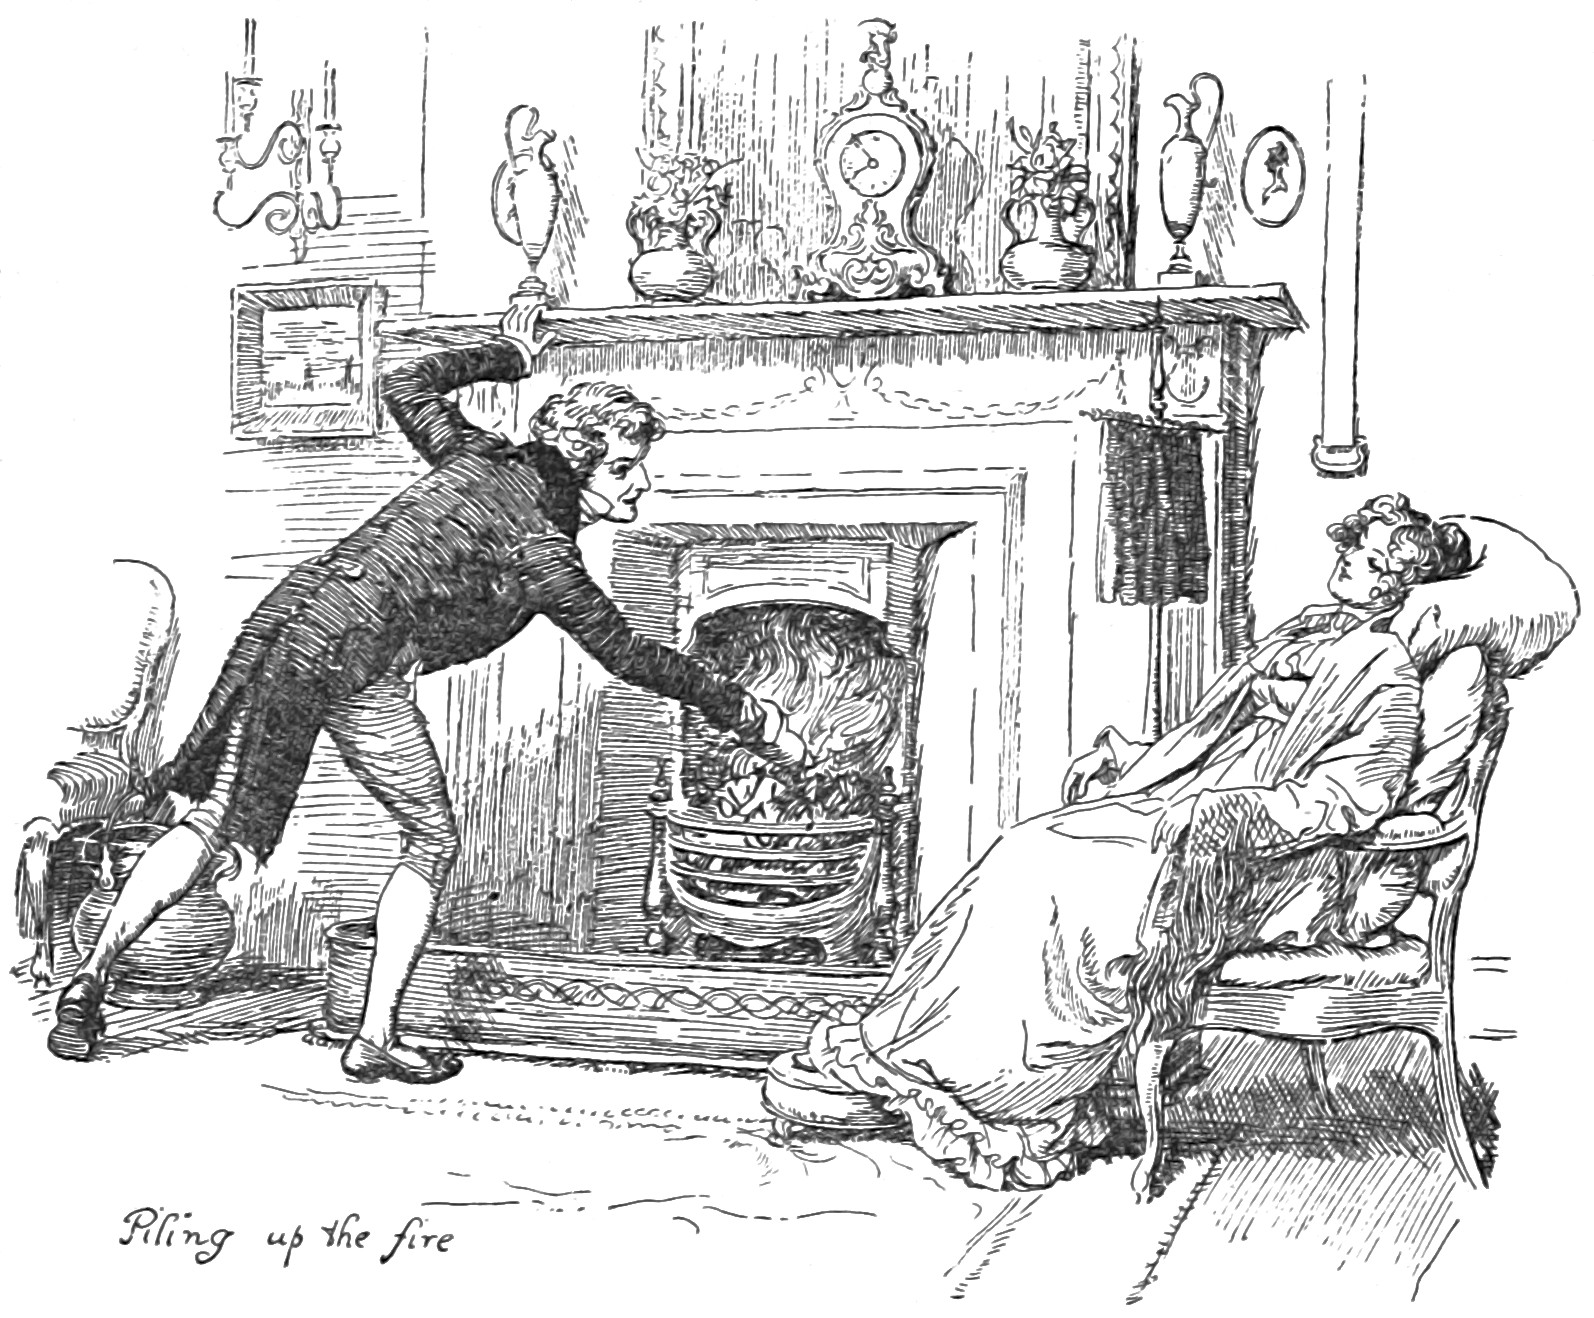
\includegraphics[width=.9\linewidth]{11fire}
\captionlistentry{Piling up the fire}
\end{figure}

	\lettrine[lines=6,image=true]{initials/chap11w}{hen}  the ladies removed after dinner Elizabeth ran up to her sister, and seeing her well guarded from cold, attended her into the drawing-room, where she was welcomed by her two friends with many professions of pleasure; and Elizabeth had never seen them so agreeable as they were during the hour which passed before the gentlemen appeared. Their powers of conversation were considerable. They could describe an entertainment with accuracy, relate an anecdote with humour, and laugh at their acquaintance with spirit.

But when the gentlemen entered, Jane was no longer the first object; Miss Bingley's eyes were instantly turned towards Darcy, and she had something to say to him before he had advanced many steps. He addressed himself directly to Miss Bennet with a polite congratulation; Mr Hurst also made her a slight bow, and said he was »very glad;« but diffuseness and warmth remained for Bingley's salutation. He was full of joy and attention. The first half hour was spent in piling up the fire, lest she should suffer from the change of room; and she removed, at his desire, to the other side of the fireplace, that she might be farther from the door. He then sat down by her, and talked scarcely to anyone else. Elizabeth, at work in the opposite corner, saw it all with great delight.

%\begin{figure}[tbph]
%\centering
%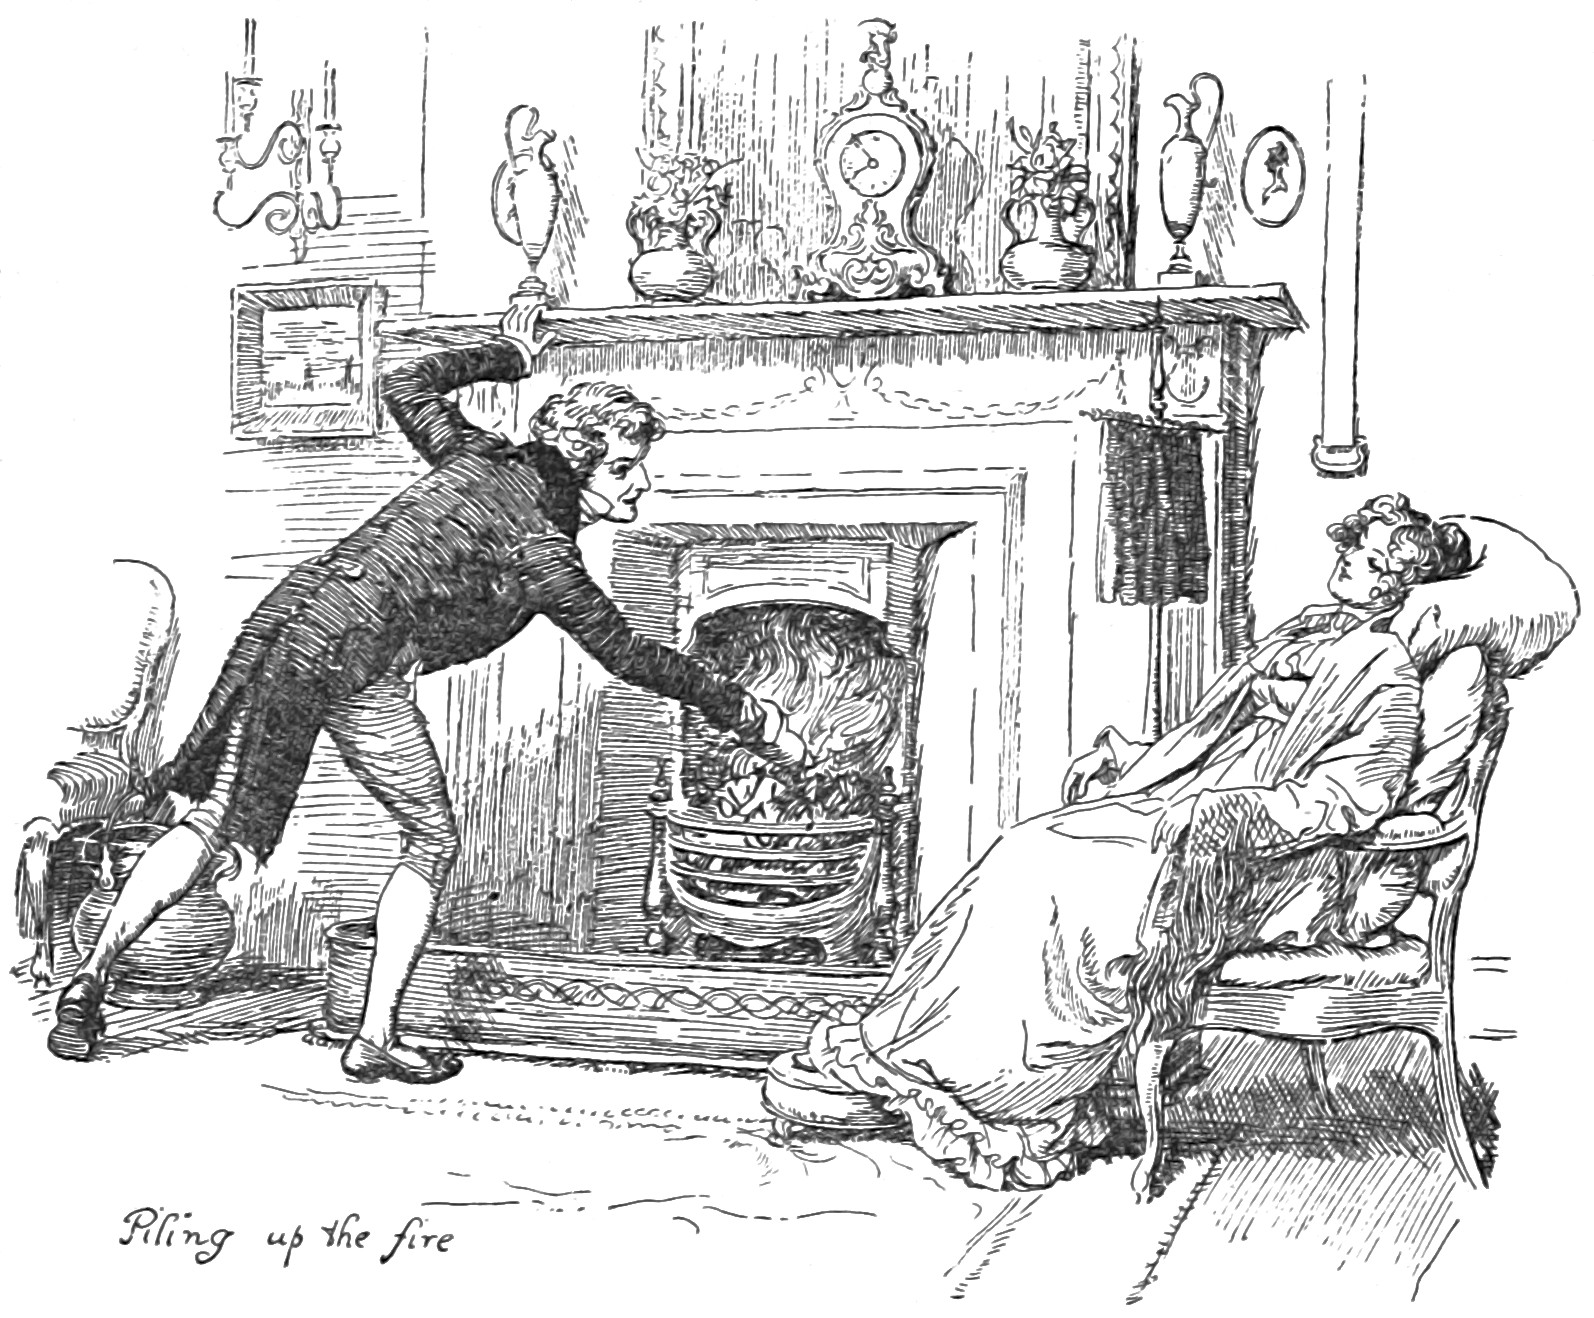
\includegraphics[width=.8\linewidth]{11fire}
%\captionlistentry{»Piling up the fire«}
%\end{figure}

When tea was over Mr Hurst reminded his sister-in-law of the card-table—but in vain. She had obtained private intelligence that Mr Darcy did not wish for cards, and Mr Hurst soon found even his open petition rejected. She assured him that no one intended to play, and the silence of the whole party on the subject seemed to justify her. Mr Hurst had, therefore, nothing to do but to stretch himself on one of the sofas and go to sleep. Darcy took up a book. Miss Bingley did the same; and Mrs Hurst, principally occupied in playing with her bracelets and rings, joined now and then in her brother's conversation with Miss Bennet.

Miss Bingley's attention was quite as much engaged in watching Mr Darcy's progress through \textit{his} book, as in reading her own; and she was perpetually either making some inquiry, or looking at his page. She could not win him, however, to any conversation; he merely answered her question and read on. At length, quite exhausted by the attempt to be amused with her own book, which she had only chosen because it was the second volume of his, she gave a great yawn and said, »How pleasant it is to spend an evening in this way! I declare, after all, there is no enjoyment like reading! How much sooner one tires of anything than of a book! When I have a house of my own, I shall be miserable if I have not an excellent library.«

No one made any reply. She then yawned again, threw aside her book, and cast her eyes round the room in quest of some amusement; when, hearing her brother mentioning a ball to Miss Bennet, she turned suddenly towards him and said,—

»By the bye Charles, are you really serious in meditating a dance at Netherfield? I would advise you, before you determine on it, to consult the wishes of the present party; I am much mistaken if there are not some among us to whom a ball would be rather a punishment than a pleasure.«

»If you mean Darcy,« cried her brother, »he may go to bed, if he chooses, before it begins; but as for the ball, it is quite a settled thing, and as soon as Nicholls has made white soup enough I shall send round my cards.«

»I should like balls infinitely better,« she replied, »if they were carried on in a different manner; but there is something insufferably tedious in the usual process of such a meeting. It would surely be much more rational if conversation instead of dancing made the order of the day.«

»Much more rational, my dear Caroline, I dare say; but it would not be near so much like a ball.«

Miss Bingley made no answer, and soon afterwards got up and walked about the room. Her figure was elegant, and she walked well; but Darcy, at whom it was all aimed, was still inflexibly studious. In the desperation of her feelings, she resolved on one effort more; and, turning to Elizabeth, said,—

»Miss Eliza Bennet, let me persuade you to follow my example, and take a turn about the room. I assure you it is very refreshing after sitting so long in one attitude.«

Elizabeth was surprised, but agreed to it immediately. Miss Bingley succeeded no less in the real object of her civility: Mr Darcy looked up. He was as much awake to the novelty of attention in that quarter as Elizabeth herself could be, and unconsciously closed his book. He was directly invited to join their party, but he declined it, observing that he could imagine but two motives for their choosing to walk up and down the room together, with either of which motives his joining them would interfere. What could he mean? She was dying to know what could be his meaning—and asked Elizabeth whether she could at all understand him.

»Not at all,« was her answer; »but, depend upon it, he means to be severe on us, and our surest way of disappointing him will be to ask nothing about it.«

Miss Bingley, however, was incapable of disappointing Mr Darcy in anything, and persevered, therefore, in requiring an explanation of his two motives.

»I have not the smallest objection to explaining them,« said he, as soon as she allowed him to speak. »You either choose this method of passing the evening because you are in each other's confidence, and have secret affairs to discuss, or because you are conscious that your figures appear to the greatest advantage in walking: if the first, I should be completely in your way; and if the second, I can admire you much better as I sit by the fire.«

»Oh, shocking!« cried Miss Bingley. »I never heard anything so abominable. How shall we punish him for such a speech?«

»Nothing so easy, if you have but the inclination,« said Elizabeth. »We can all plague and punish one another. Tease him—laugh at him. Intimate as you are, you must know how it is to be done.«

»But upon my honour I do \textit{not}. I do assure you that my intimacy has not yet taught me \textit{that}. Tease calmness of temper and presence of mind! No, no; I feel he may defy us there. And as to laughter, we will not expose ourselves, if you please, by attempting to laugh without a subject. Mr Darcy may hug himself.«

»Mr Darcy is not to be laughed at!« cried Elizabeth. »That is an uncommon advantage, and uncommon I hope it will continue, for it would be a great loss to \textit{me} to have many such acquaintance. I dearly love a laugh.«

»Miss Bingley,« said he, »has given me credit for more than can be. The wisest and best of men,—nay, the wisest and best of their actions,—may be rendered ridiculous by a person whose first object in life is a joke.«

»Certainly,« replied Elizabeth, »there are such people, but I hope I am not one of \textit{them}. I hope I never ridicule what is wise or good. Follies and nonsense, whims and inconsistencies, \textit{do} divert me, I own, and I laugh at them whenever I can. But these, I suppose, are precisely what you are without.«

»Perhaps that is not possible for anyone. But it has been the study of my life to avoid those weaknesses which often expose a strong understanding to ridicule.«

»Such as vanity and pride.«

»Yes, vanity is a weakness indeed. But pride—where there is a real superiority of mind—pride will be always under good regulation.«

Elizabeth turned away to hide a smile.

»Your examination of Mr Darcy is over, I presume,« said Miss Bingley; »and pray what is the result?«

»I am perfectly convinced by it that Mr Darcy has no defect. He owns it himself without disguise.«

»No,« said Darcy, »I have made no such pretension. I have faults enough, but they are not, I hope, of understanding. My temper I dare not vouch for. It is, I believe, too little yielding; certainly too little for the convenience of the world. I cannot forget the follies and vices of others so soon as I ought, nor their offences against myself. My feelings are not puffed about with every attempt to move them. My temper would perhaps be called resentful. My good opinion once lost is lost for ever.«

»\textit{That} is a failing, indeed!« cried Elizabeth. »Implacable resentment \textit{is} a shade in a character. But you have chosen your fault well. I really cannot \textit{laugh} at it. You are safe from me.«

»There is, I believe, in every disposition a tendency to some particular evil, a natural defect, which not even the best education can overcome.«

»And \textit{your} defect is a propensity to hate everybody.«

»And yours,« he replied, with a smile, »is wilfully to misunderstand them.«

»Do let us have a little music,« cried Miss Bingley, tired of a conversation in which she had no share. »Louisa, you will not mind my waking Mr Hurst.«

Her sister made not the smallest objection, and the pianoforte was opened; and Darcy, after a few moments' recollection, was not sorry for it. He began to feel the danger of paying Elizabeth too much attention.